
\chapter{Experimental Results}
\label{chap:exp}

This chapter presents the experiments and the results for the evaluation of the following methods: a proposed robot-camera calibration method and the 3D object pose estimation method. As to the robot-camera calibration method, the internal parameters of the camera need to be estimated. Methods for estimating the internal parameters, also known as intrinsic parameters of the camera already exists and two of the most popular methods available in the open-source community were selected. A detailed description of these methods is in Chapter \ref{chap:robot}. In order to validate the output of the intrinsic parameters, a reprojection error as a metric is selected in this thesis. Then, with the most accurate internal parameters, the camera-robot calibration proceeds. A repeatability test, as a validation test for the result of the robot-camera calibration follows the calibration step. Finally, with the most accurate result of the robot-camera calibration, experiments for testing the 3D pose estimation system starts. For the purpose of testing, an industrial object is required as well as its CAD model. The latter is accomplished with the use of the FreeCAD software \ref{freecadb}, then, a suitable scaling undergoes with the use of CloudCompare software \ref{cloudcompareb}, where a point cloud is generated. As to the validation of the method, a ground truth of the object needs to be known in advance. For such a requirement a checkerboard is used as described in Figure \ref{setupsystem1} and Figure \ref{setupsystem2}. By placing the robot TCP at specific points (three points in total), the checkerboard can be localized and a new workobject is produced. The checkboard workspace is used to determine the ground-truth of the object pose which is compared with the 3D object pose estimation system described in Chapter \ref{chap:theo}. The system is evaluated by analyzing the translation and rotation errors. 

\begin{figure}[htp]
\begin{center}
{
  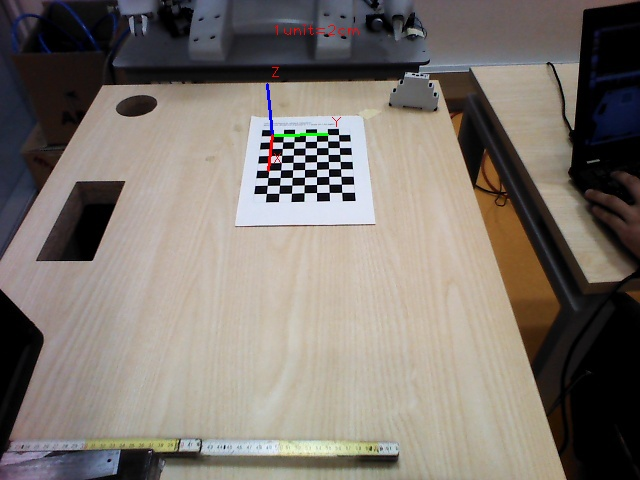
\includegraphics[clip,width=0.7\columnwidth]{images/setup3.jpg}
}
\end{center}
\begin{center}
{
  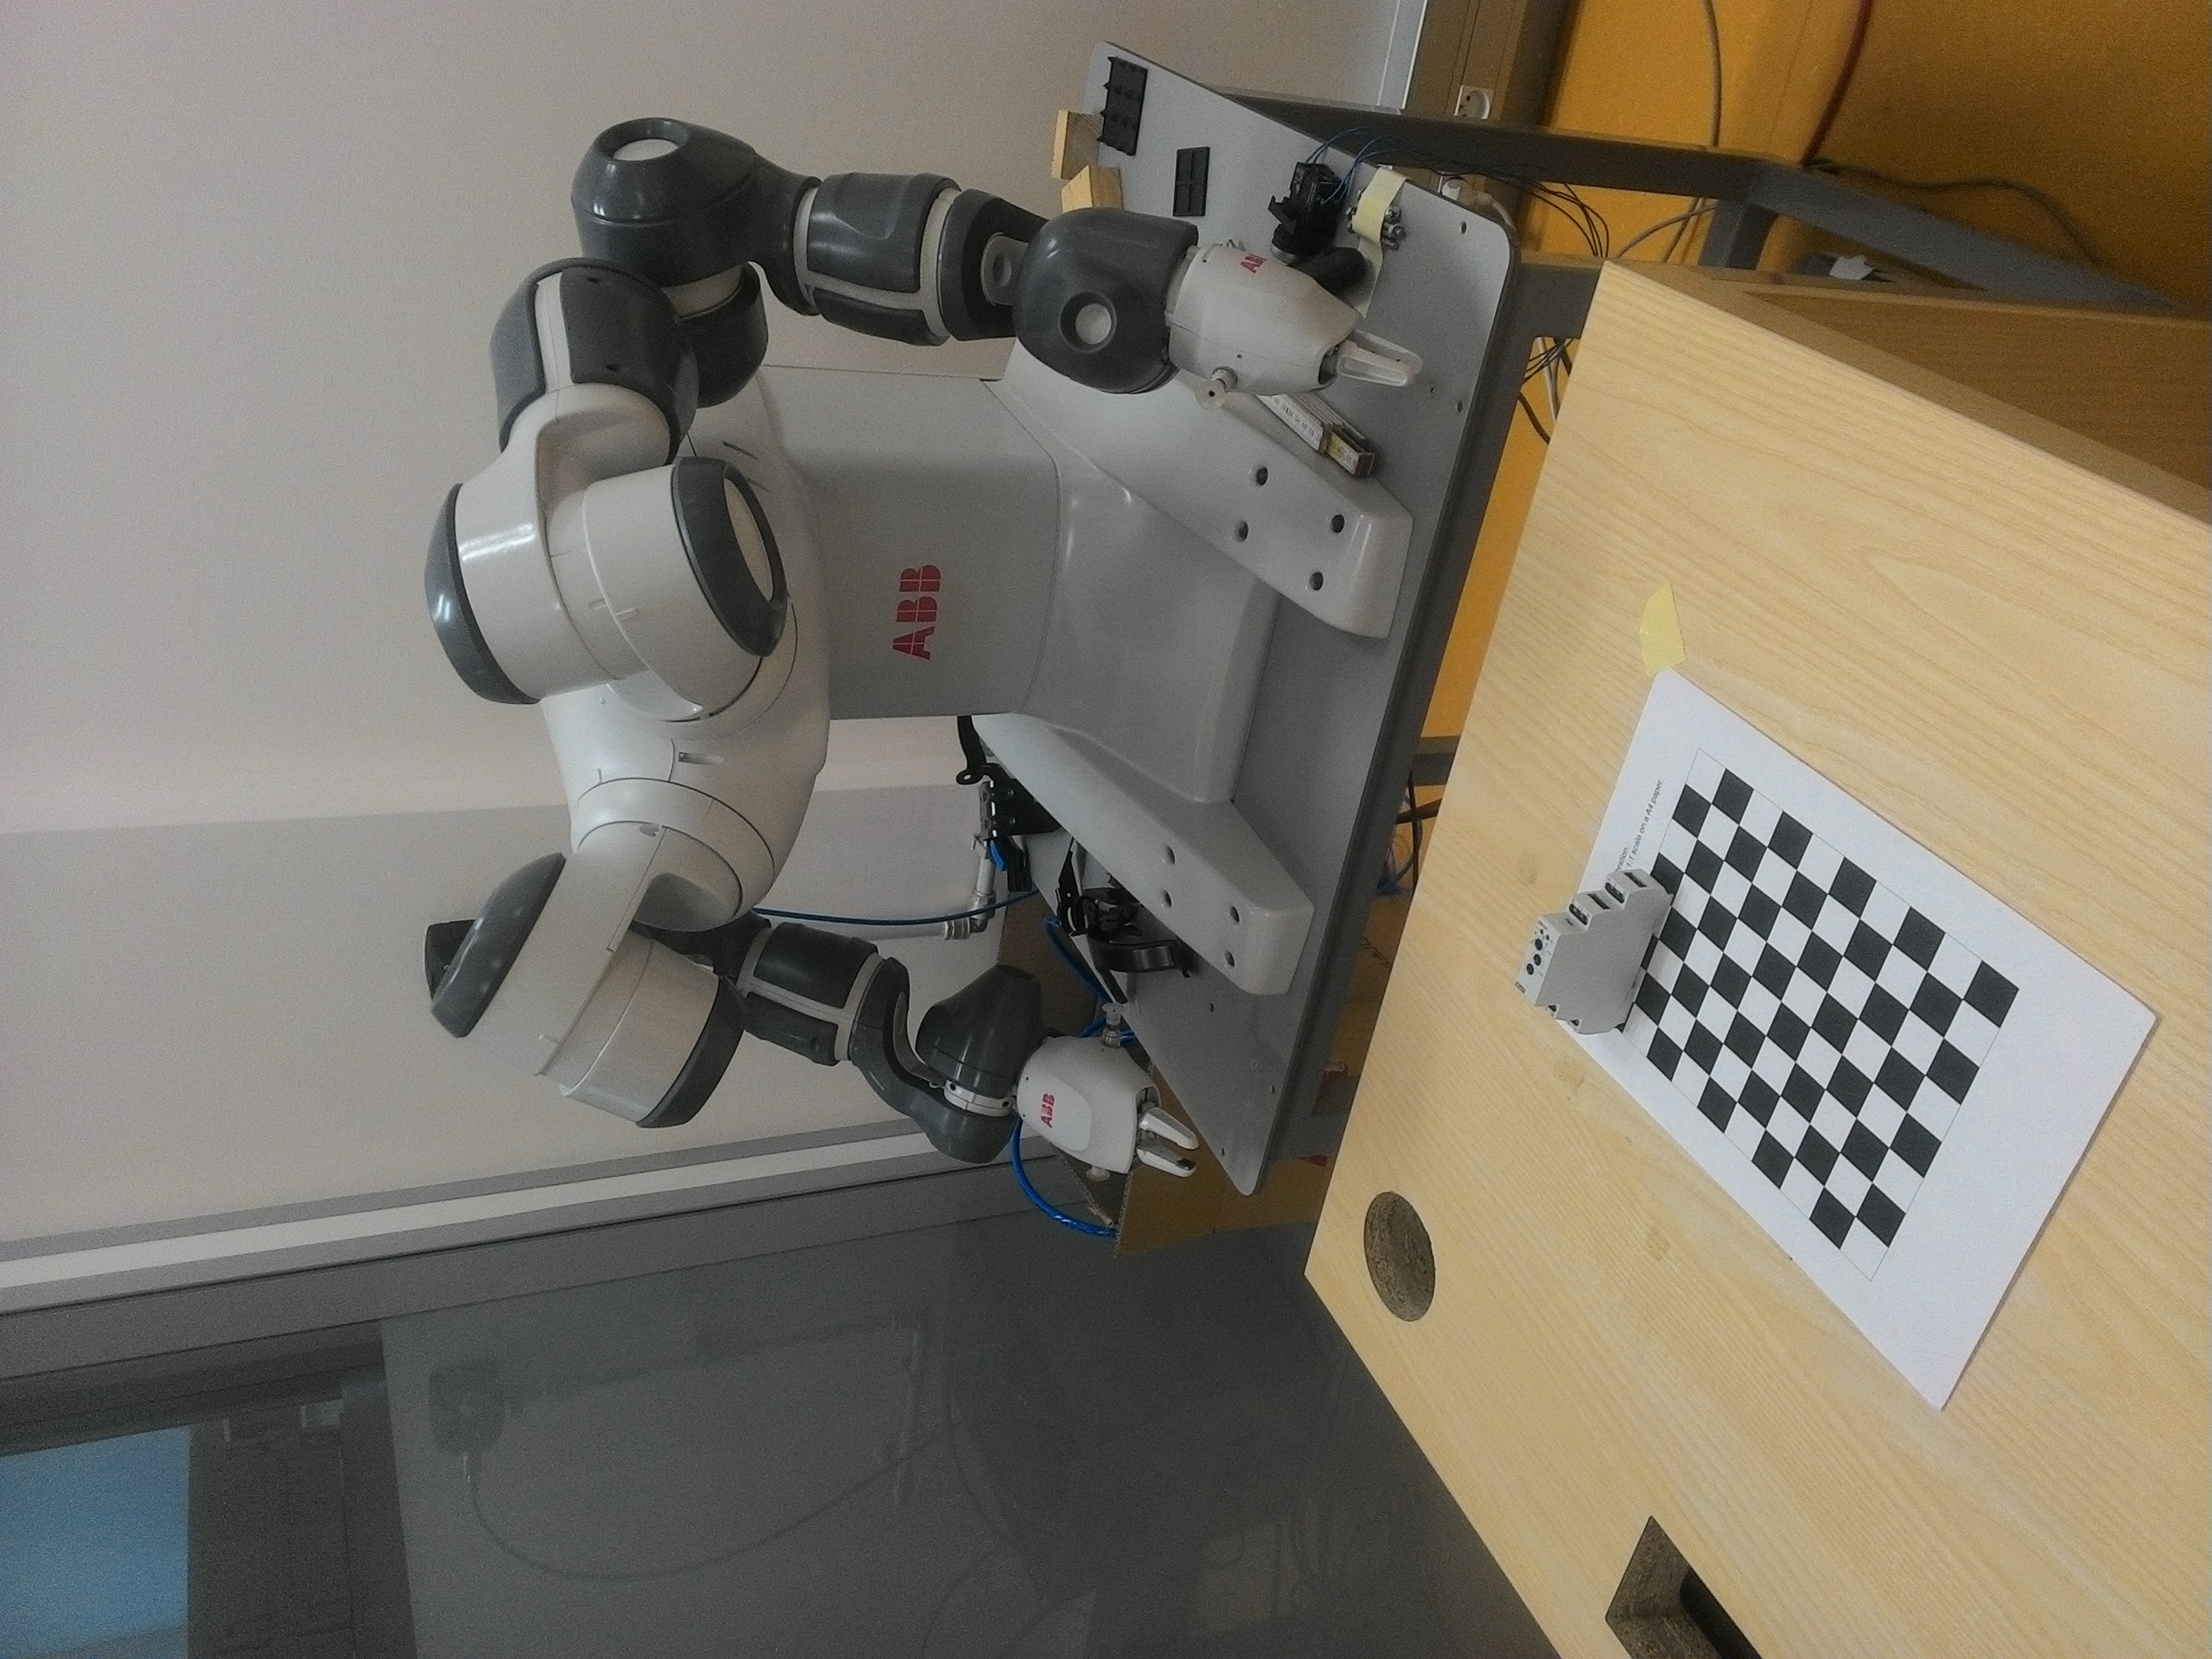
\includegraphics[clip,width=0.7\columnwidth]{images/setup2.png}
}
\end{center}

\caption{Overview of the Validation System: Checkerboard placement.}
\label{setupsystem1}
\end{figure}



\begin{figure}[htp]
\begin{center}
{
  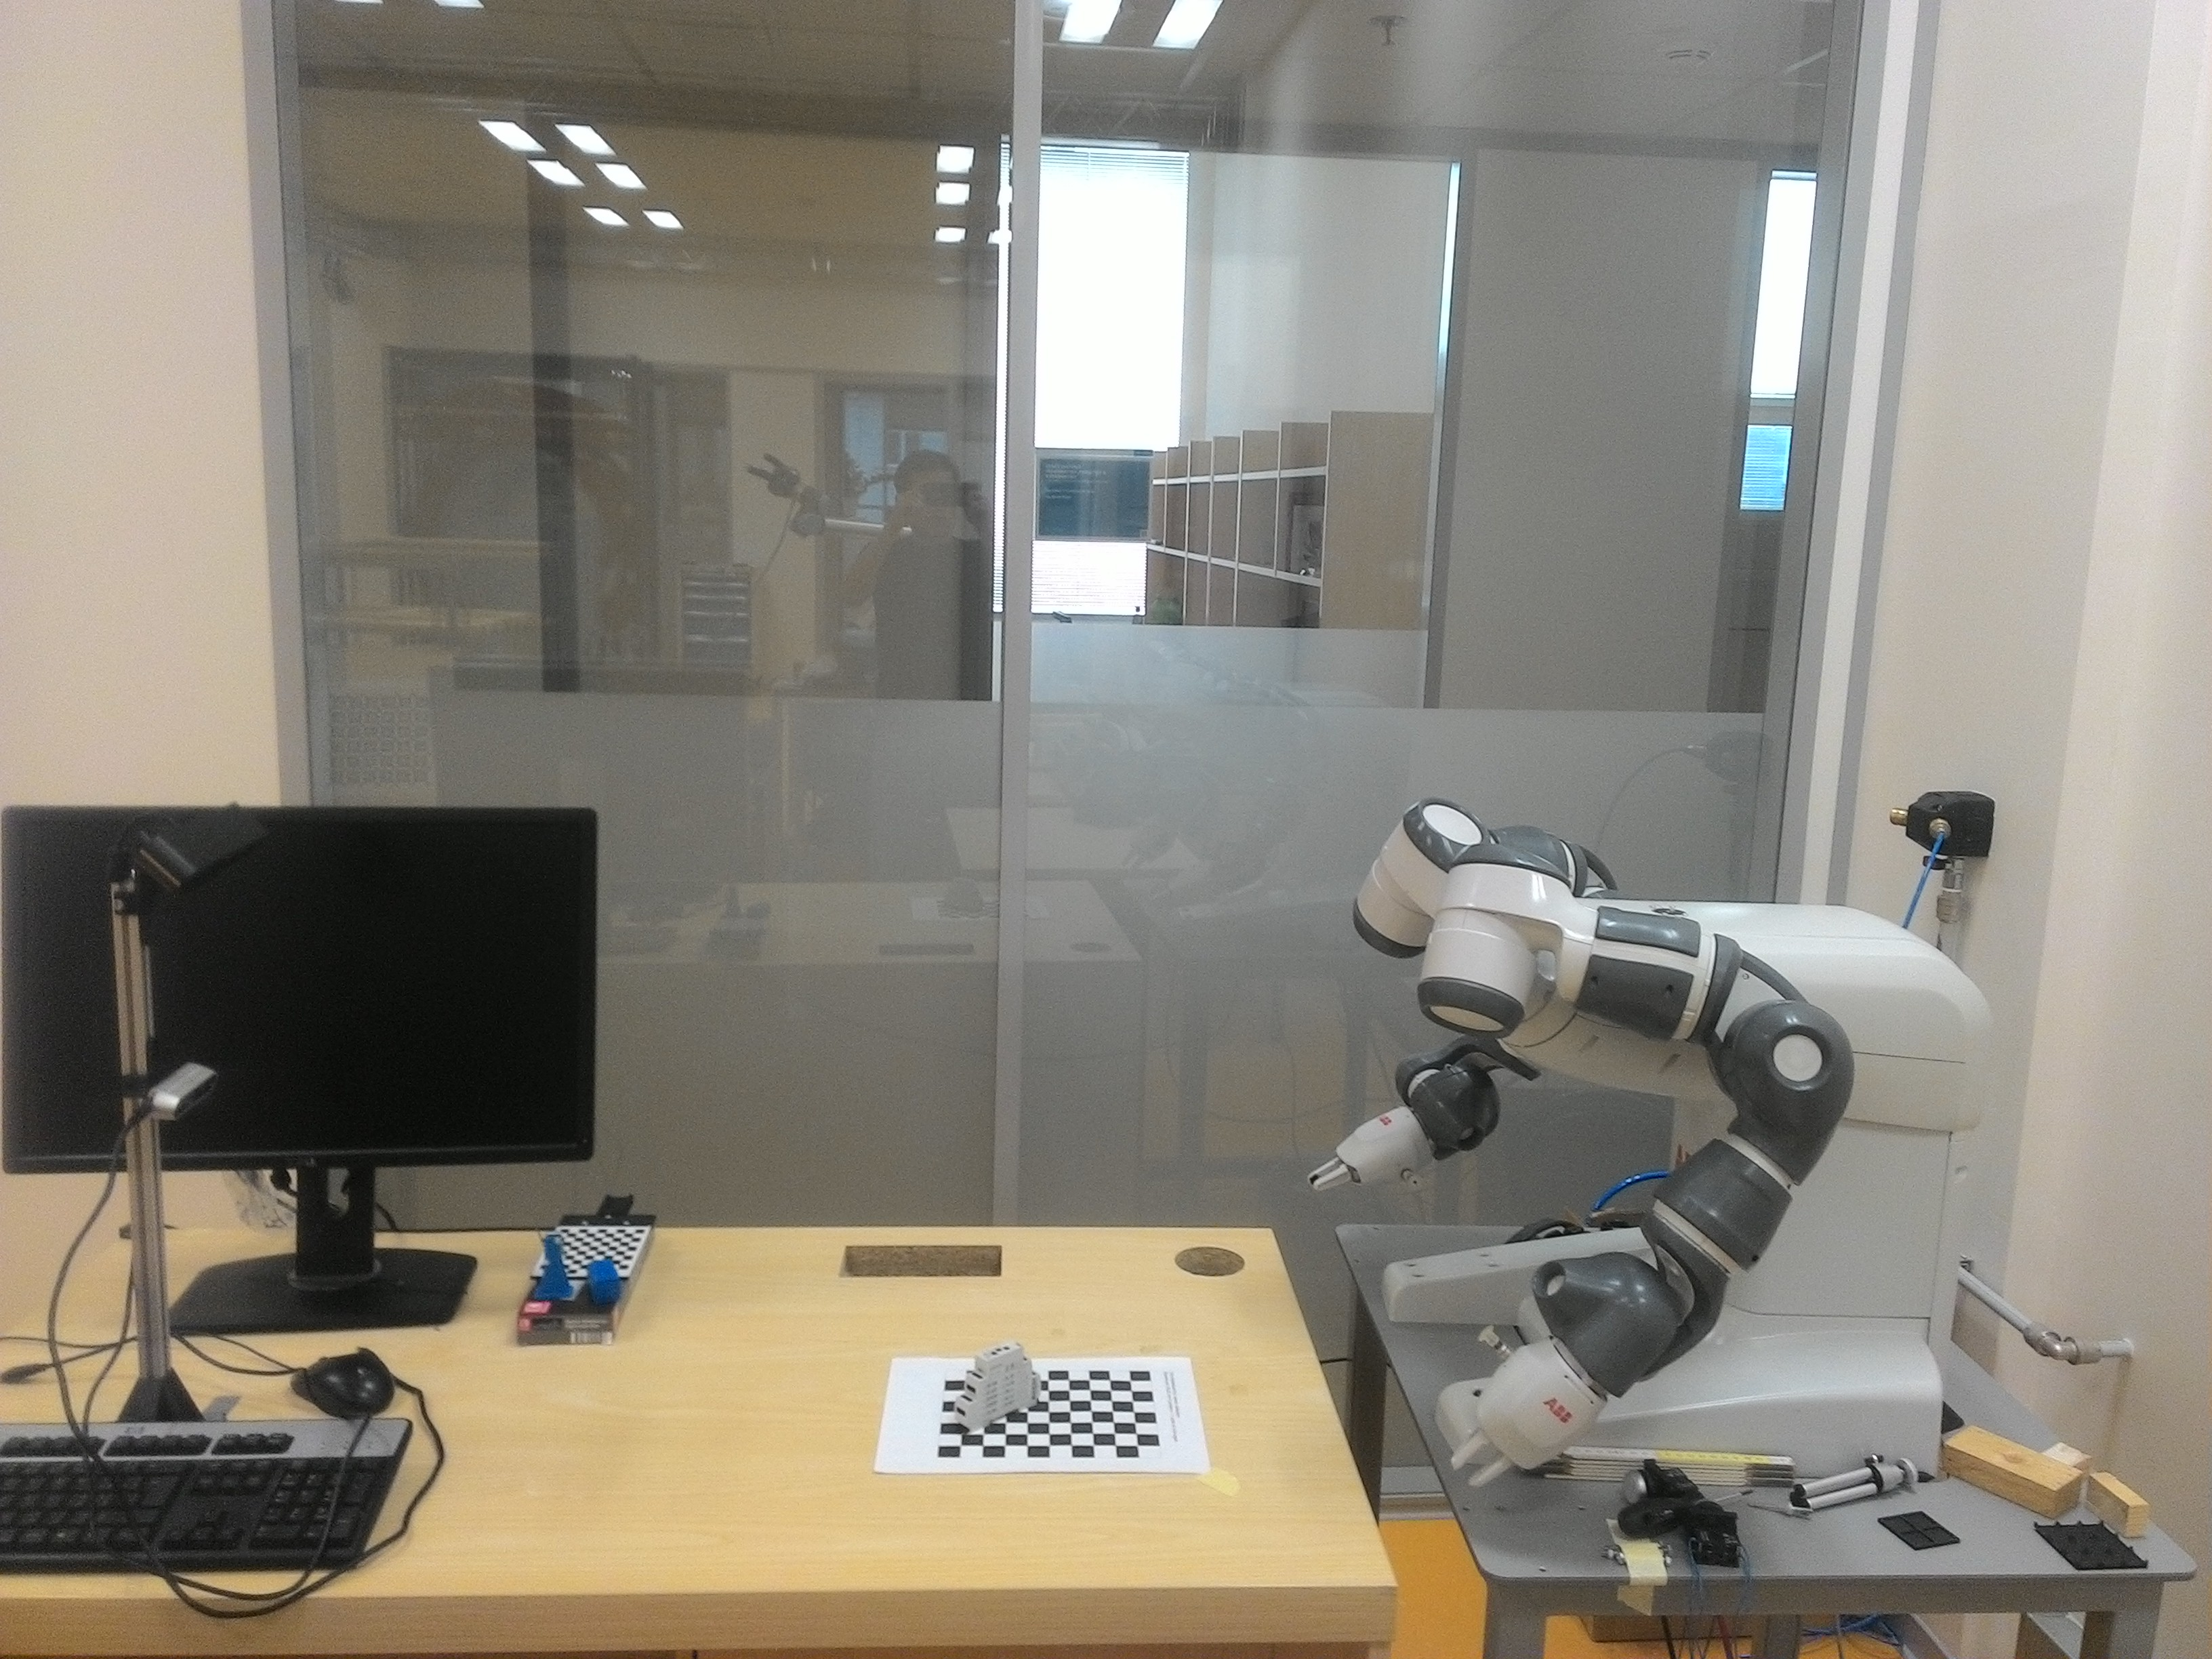
\includegraphics[clip,width=0.7\columnwidth]{images/setup1.jpg}
}
\end{center}
\begin{center}
{
  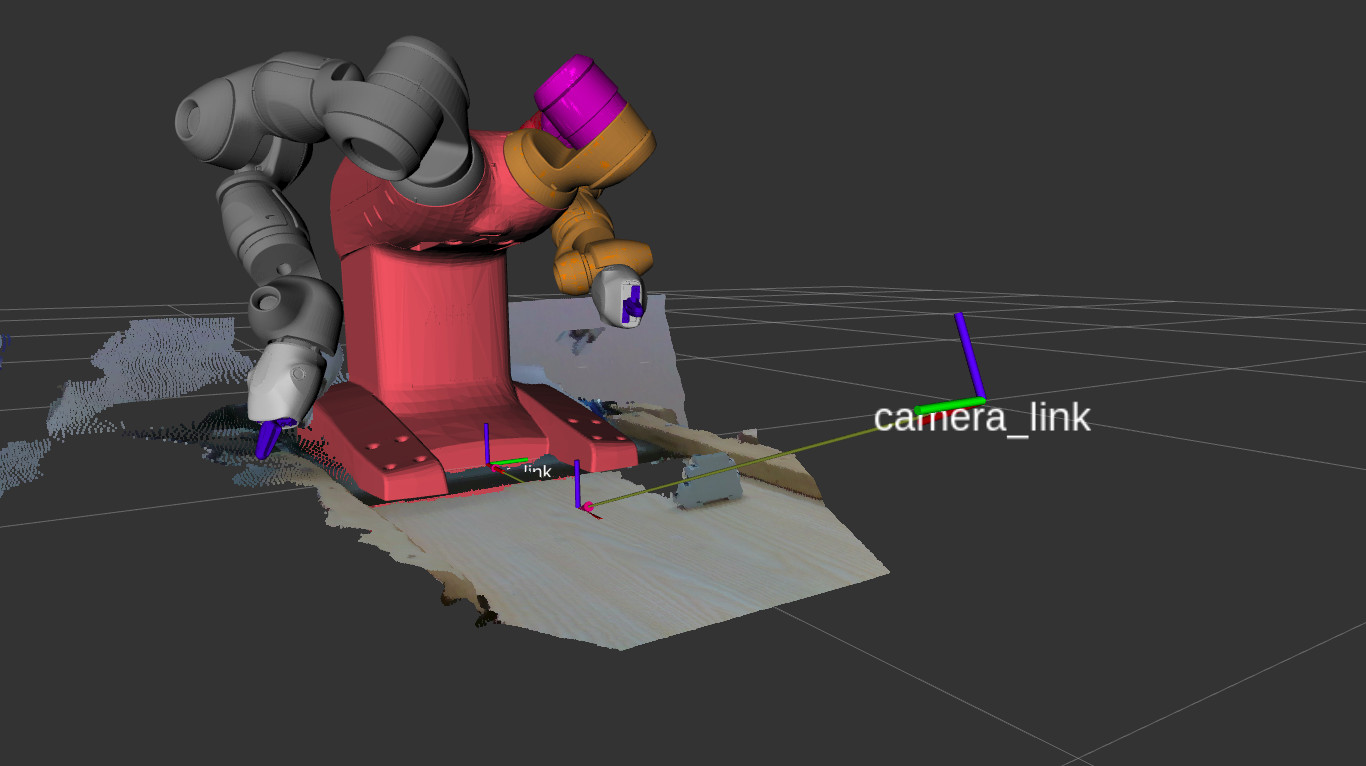
\includegraphics[clip,width=0.7\columnwidth]{images/system1.jpg}
}
\end{center}
\caption{Overview of the Validation System: Checkerboard placement and Visualization in Rviz simulator.}
\label{setupsystem2}
\end{figure}


\section{Robot-Camera Calibration on the YuMi Robot}

In order to get the most accurate estimation of the robot-camera pose, careful attention must be given to the internal parameters of the camera which is a determining factor when determining the accuracy of the extrinsic parameters. For such estimation of those parameters, two methods were selected and a detailed description of both is shown in Chapter \ref{chap:robot}. An Astra camera and a RealSense D-435 camera are used in this thesis. The cameras are calibrated with the methods previously mentioned and their results are shown in \ref{chap:intpara}. As to the validation process, a reprojection error is used. Since it is one of the most used metrics,  it is used in this thesis. 

\subsection{Reprojection Error}

The reprojection error is the distance between a pattern keypoint detected in a calibration image and a corresponding world point projected into the same image. Figure \ref{fig:realopen} and Figure \ref{fig:realros} show the calibration results by analyzing the reprojection error per image using a RealSense D-435 camera with the OpenCV and camera\textunderscore industrial calibration methods. Figure \ref{fig:astraopen} and Figure \ref{fig:astraros} show the calibration results by analyzing the reprojection error per image using an Astra camera. The results were analyzed using the reprojection error per image with both methods: the OpenCV and camera\textunderscore industrial calibration.



%%%%%%%%%%%%%%%%%%%%%%%%%%%%%%%%%%%%%%%%%%
\begin{figure}[!h]
\begin{center}
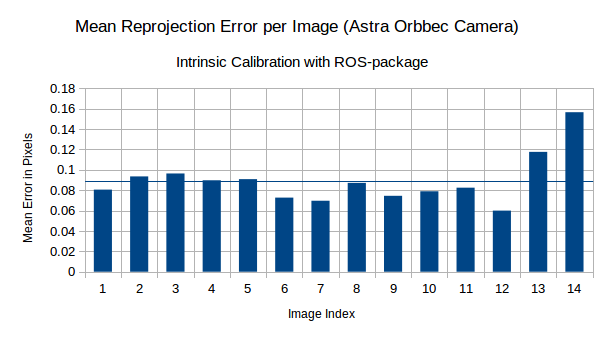
\includegraphics[width=5in, height=3.5in]{figures05/int/ros_int_cal_astra.png}
\caption{Mean Reprojection Error per Image with the ROS Method (Astra Orbbec Camera)}%\cite{temp2}}
\label{fig:astraros}
\end{center}
\end{figure}

\begin{figure}[!h]
\begin{center}
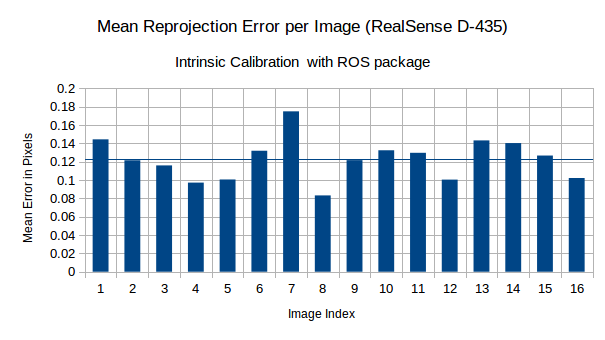
\includegraphics[width=5in, height=3.5in]{figures05/int/ros_int_cal_real.png}
\caption{Mean Reprojection Error per Image with the ROS Method (RealSense D-435)}%\cite{temp2}}
\label{fig:realros}
\end{center}
\end{figure}

\begin{figure}[!h]
\begin{center}
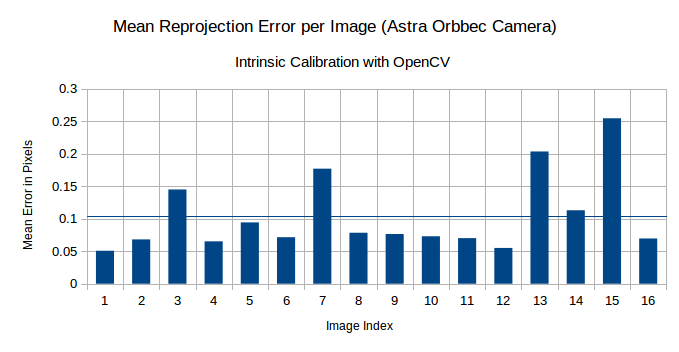
\includegraphics[width=5in, height=3.5in]{figures05/int/opencv_int_cal_astra.png}
\caption{Mean Reprojection Error per Image with the OpenCV Method (Astra Orbbec Camera)}%\cite{temp2}}
\label{fig:astraopen}
\end{center}
\end{figure}

\begin{figure}[!h]
\begin{center}
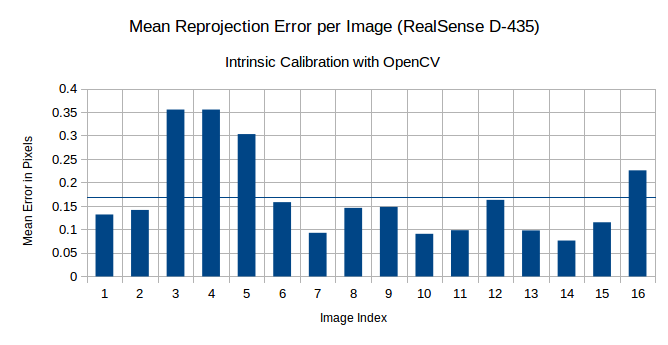
\includegraphics[width=5in, height=3.5in]{figures05/int/opencv_int_cal_real.png}
\caption{Mean Reprojection Error per Image with the OpenCV Method (RealSense D-435)}%\cite{temp2}}
\label{fig:realopen}
\end{center}
\end{figure}

In order to discuss the results for each case, an average error is calculated. This is done by computing the arithmetical mean of the errors calculated for all the calibration images. And that result should be as close to zero as possible according to the literature in computer vision.

\subsection{Result Analysis}
After computing the average error for both cameras, the results are shown in Table \ref{astra1} for the Astra camera and Table \ref{real1} which is for the RealSense D-435.\\
 As seen in Figure \ref{fig:astraros} and Figure \ref{fig:astraopen}, the overall mean errors of the Astra camera computed for both method are correlated to each other. The reprojection error was obtained from OpenCV and camera\textunderscore industrial calibration, which showed very similar figures with only a small offset. This difference is acceptable. The requirement is to be under 0.5 pixels, a specified value accepted as determining how accurate a device sensor is. \\
 
On the other hand, the results for the RealSense camera are not as closely correlated to one another method. The sensor might be more sensitive to small movement in the calibration target resulting in taking wrong measurements. In addition to that, the light condition can also affect the sensory device since the data taken is an RGB image. Such a difference presented in the mean reprojection error can largely affect the output accuracy of the estimation of the camera frame relative to the robot frame by applying the eye-to-hand calibration. In order to confirm that this difference holds we proceeded to take new measurements, without moving the calibration target when the sensory device is taking its sample. Then the whole process is evaluated again. The difference holds between methods, but meet the requirements of being under 0.5 pixels. With the results it is too early to conclude the effectiveness of the RealSense D-435 camera. Keeping this difference in mind, we proceed with the next experiment for validating the robot-camera calibration.  \\
Both cameras were calibrated with the same light conditions, calibration target and an equal number of images. Considering all of this, it can be concluded that the Astra camera seems to perform well and it can be our final choice for the pose estimation system evaluation. 

\begin{table}[ht]
\renewcommand{\arraystretch}{1.3}
\caption{Experimental data for internal Astra sensor calibration.}
\label{astra1}
\centering
\begin{tabular}{|c||c|}
\hline
Method & Overall Mean Error (pixels)\\
\hline
OpenCV &  0.1041954808\\
\hline
ROS &  0.1081118023\\
\hline
\end{tabular}
\end{table}

\begin{table}[ht]
\renewcommand{\arraystretch}{1.3}
\caption{Experimental data for internal RealSense sensor calibration.}
\label{real1}
\centering
\begin{tabular}{|c||c|}
\hline
Method & Overall Mean Error (pixels)\\
\hline
OpenCV &  0.1684388411\\
\hline
ROS &  0.122868849\\
\hline
\end{tabular}
\end{table}

\subsection{Eye-To-Hand Calibration}

The second experiment in this Chapter \ref{chap:exp} is related to the eye-to-hand calibration. In this experiment, both cameras, the Astra and RealSense D-435, are used for the validation test. Since the quality of the extrinsic calibration depends on how good the estimation of the internal parameters is, we proceed with taking the most accurate internal parameters based on the reprojection error as described previously. \\
By defining the best internal parameters, the validation test is divided into two types. In the first part of the experiment, the calibration plate with a checkerboard placed on it as described in Chapter \ref{chap:robot} is kept at a constant angle, parallel to the XY plane of the robot coordinate system. Figure \ref{setupext1} shows the basic setup for the extrinsic calibration with a constant orientation parallel to the XY plane of the robot. The whole process includes movements with a small offset between every pose of the TCP (Tool Center Point). The joint configuration values for each pose is known in advance. Each pose guarantees that the checkerboard is detected by the robot. Basically, the robot executes a translation of the calibration target in its XY plane.\\ 

As to the second part of the experiment, the calibration plate is not kept at  a constant angle, but is tilted with predefined orientations provided that the checkerboard is always detected by the camera. Figure \ref{setupext2} shows the basic setup for the extrinsic calibration with tilting motion. After defining the type of movement, several criteria for obtaining a reasonable estimation of the camera relative to the robot frame are taken into account. One of the considerations is to pause for few seconds among the movements. This is with the aim to cancel the effects of possible vibrations that the robot can produce, in an attempt to avoid wrong measurement throughout the extrinsic calibration process. Another consideration is related to speed. A reasonable speed of $25\%$ is set for the validation test. \\

With the types of experiments and the main criteria to consider for each one known in advance, the execution of the robot movement can be started. To be able to control the robot arm, interface one of each camera in each test, and estimate the pose of the camera relative to the robot base, three nodes were developed as described in Chapter \ref{chap:robot}. The node named $publishingTF.py$ is responsible for controlling the robot movement and publishing the transformation from the robot frame to TCP (Tool Center Point) frame into the ROS network (tf topic to be specific). \\
The second node named $target\textunderscore locator \textunderscore astra.py$ or $target\textunderscore locator \textunderscore rsense.py$  which depends on the camera used, is responsible  for computing the estimation of the camera pose relative to the calibration target (checkerboard) frame. In addition to that, it broadcasts the estimation of camera pose into the ROS network. A third node named $listeningTF.py$ is responsible for keeping track of all the coordinate frames over time, and querying for the transformation of the camera frame relative to the robot frame.

%ASTRA
\begin{figure}[htp]
\begin{center}
{
  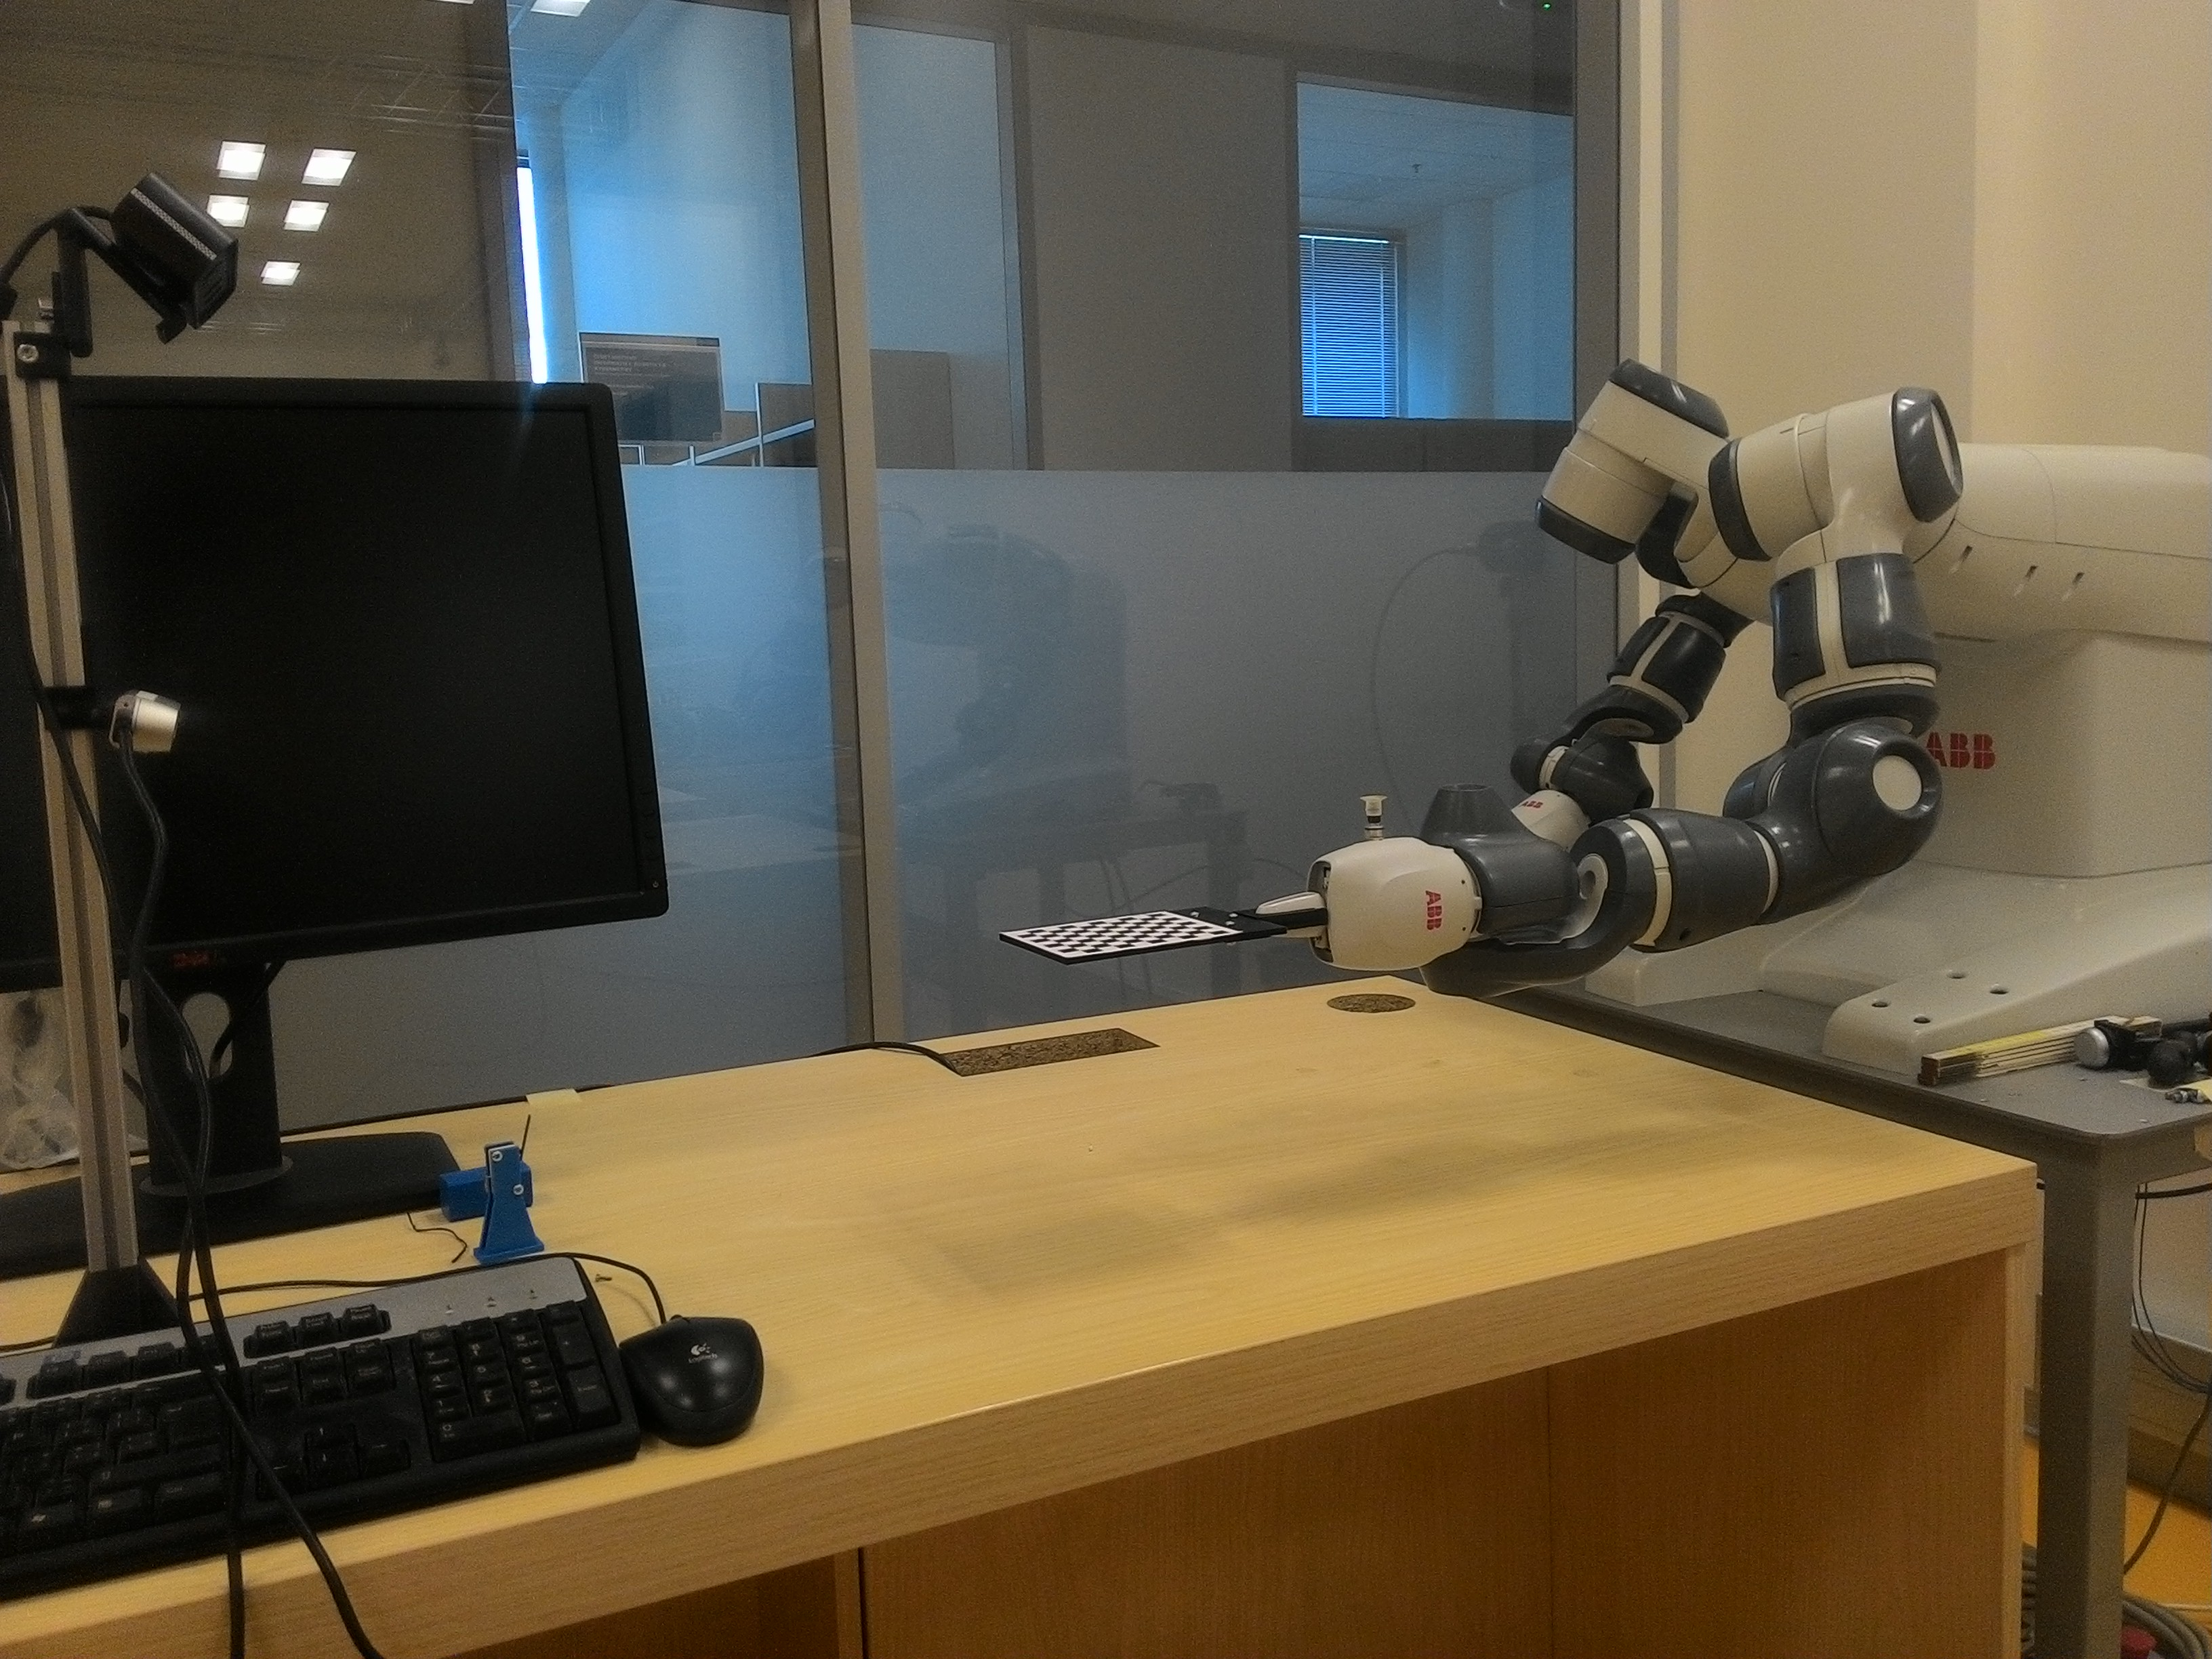
\includegraphics[clip,width=0.6\columnwidth]{images/ext1.jpg}
}
\end{center}
\begin{center}
{
  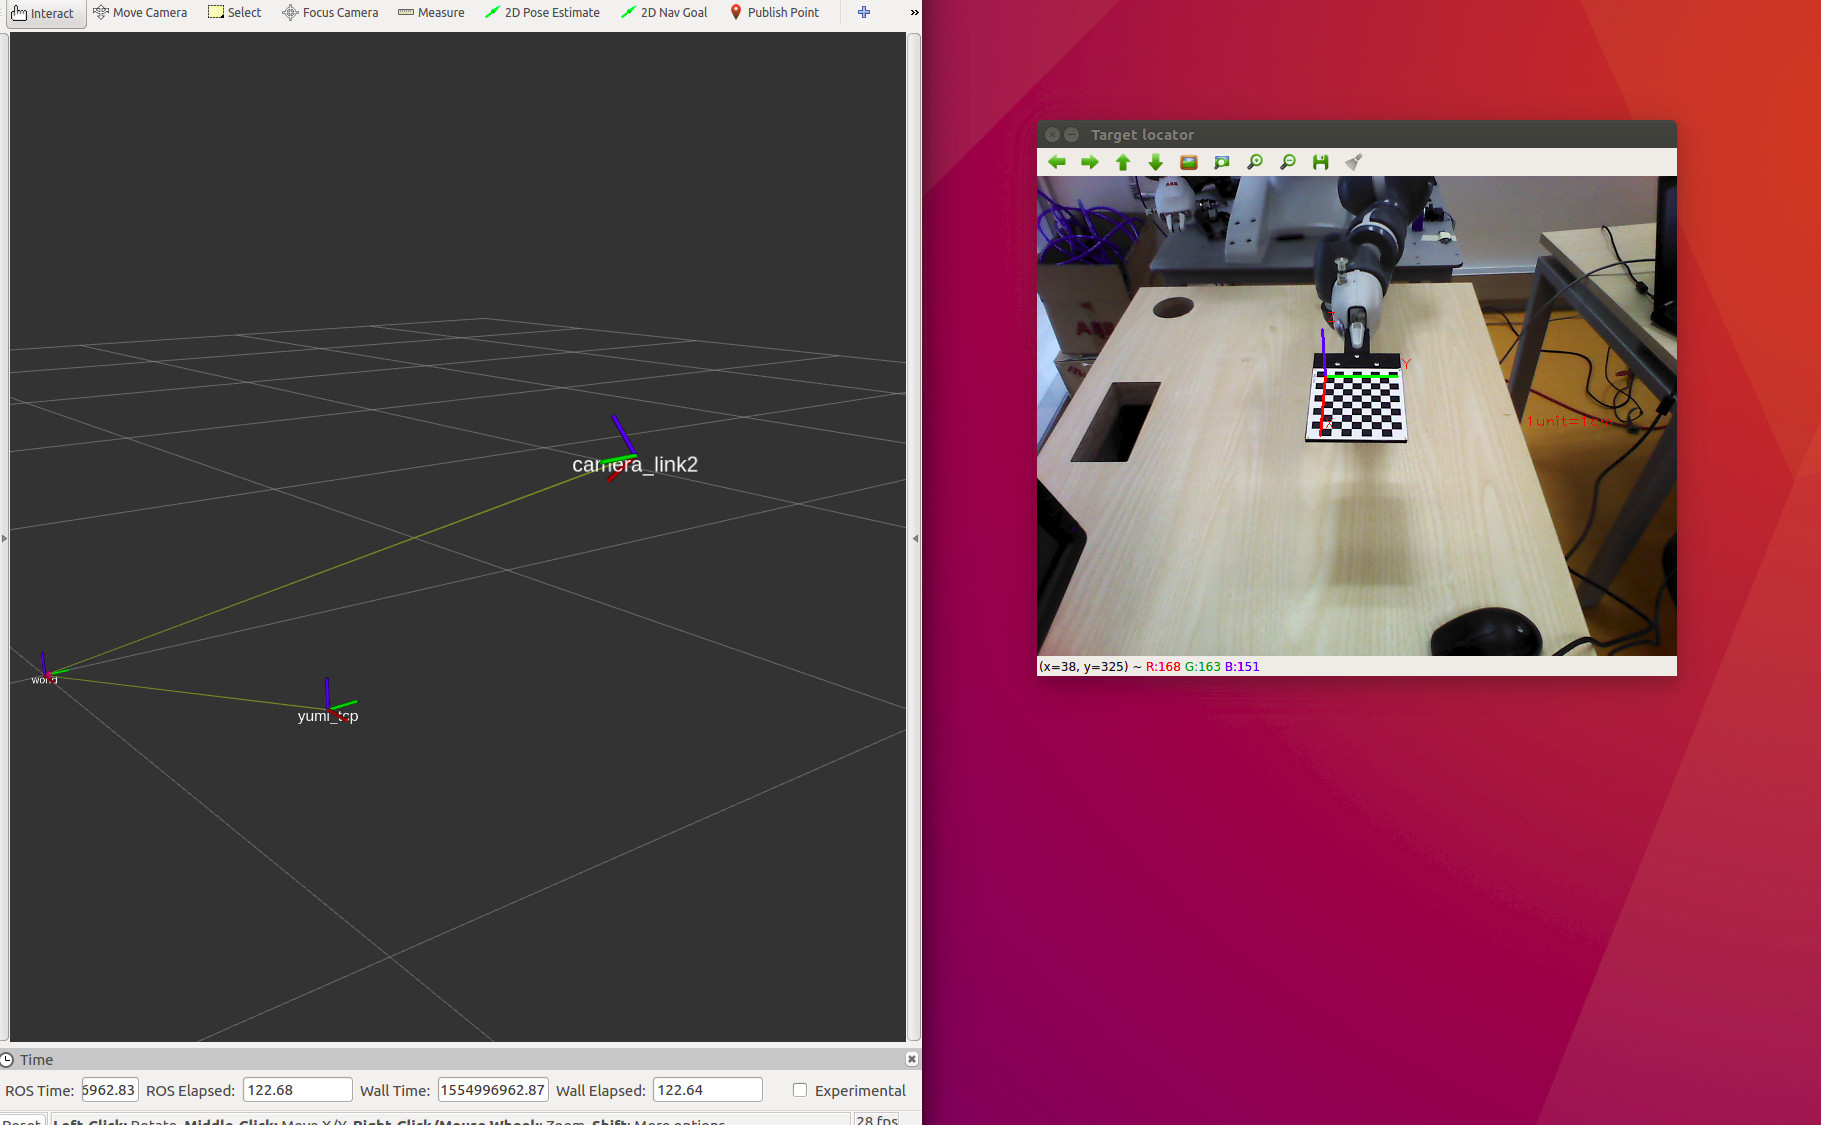
\includegraphics[clip,width=0.7\columnwidth]{images/ext2.jpg}
}
\end{center}
\caption{System setup and Visualization in Rviz of the Validation Test with a Constant Orientation.}
\label{setupext1}
\end{figure}



%%%%%%%%%
\begin{figure}[htp]
\begin{center}
{
  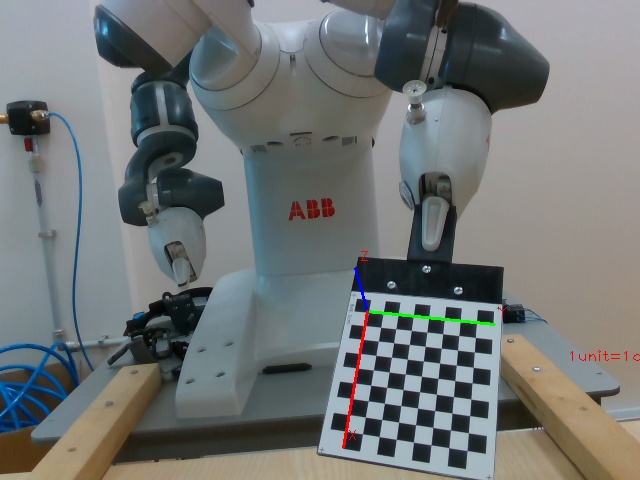
\includegraphics[clip,width=0.7\columnwidth]{images/ext3.jpg}
}
\end{center}
\begin{center}
{
  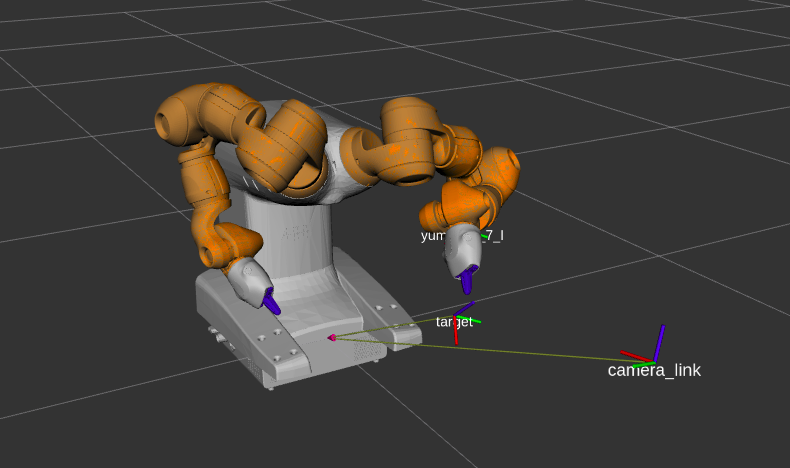
\includegraphics[clip,width=0.7\columnwidth]{images/tilting2.png}
}
\end{center}
\caption{System setup and Visualization in Rviz of the Validation Test with Tilting Motion.}
\label{setupext2}
\end{figure}


\iffalse
, as well as the computation of the average of the transformation it queries after each executed robot move. 
\fi
\subsection{Calibration results}

%%%%%%%%%%%%%%%%%%%%%%%%%%%%%%%%%% astra 
\begin{itemize}
\item The following eye-to-hand transform was obtained for the Astra Camera with the calibration plate parallel to the XY plane in robot frame:
\begin{equation}
^{R}T_{C}=\begin{bmatrix} -0.023 & 0.730 & -0.683 & 1.192\\0.999 & 0.001 & -0.032 & 0.121\\ -0.023 & -0.683 & -0.729 & 0.536 \end{bmatrix}
\end{equation}

\item The following eye-to-hand transform was obtained for the Astra Camera by tilting the calibration plate:
\begin{equation}
^{R}T_{C}=\begin{bmatrix} -0.014 & 0.724 & -0.689 & 1.195\\0.999 & -0.003 & -0.024 & 0.114\\ -0.019 & -0.689 & -0.724 & 0.536 \end{bmatrix}
\end{equation}

%%%%%%%%%%%%%%%%%%%%%%%%%%%%%%%%% realsense

\item The following eye-to-hand transform was obtained for the RealSense D-435 camera with the calibration plate parallel to the XY plane in robot frame:
\begin{equation}
^{R}T_{C}=\begin{bmatrix} -0.022 & 0.294 & -0.956 &1.223\\-0.999 & -0.001 & -0.023 & 0.118 \\ -0.007 & -0.956 & -0.294 & 0.324  \end{bmatrix}
\end{equation}

\item The following eye-to-hand transform was obtained for the RealSense D-435 camera by tilting the calibration plate:
\begin{equation}
^{R}T_{C}=\begin{bmatrix} -0.0183 & 0.309 &-0.953 & 1.219\\0.999& -0.004& -0.020& 0.094\\ -0.010& -0.953& -0.301& 0.332\end{bmatrix}
\end{equation}
\end{itemize}

\subsection{Result Analysis}

The proposed robot-camera calibration method was successfully performed provided that the calibration target was detected by the 3D camera being calibrated. In order to validate whether the proposed method is accurate enough for the pose estimation system described in Chapter \ref{chap:robot}, it is necessary to know the ground truth in advance. It was a challenge to measure an exact orientation and translation of the camera with respect to the robot frame. Such difficulty are normal to encounter since the cameras used in this thesis are not suitable for the problem to be solved. Suitable cameras for the assignment of this thesis are the so-called industrial cameras, but such camera was not available.  
For the given conditions, a validation test is still considered. A rough estimation of the camera pose relative to the robot was calculated. A measuring tape was used for the rough estimation but it is not considered as ground truth to evaluate the result of the robot-camera calibration but rather a good idea of what the result should be. \\
The repeatability test is proposed for the validation of the extrinsic parameters. It consists of repeating the whole process over again when it comes to the estimation of the external values, those that represent the camera pose relative to the robot frame. But a major difference exists. The number of the movements is increased provided that the checkerboard was detected by the camera used.

\iffalse
where the camera frame is given
given that the housing of the camera (namely the RealSense camera) is rounded 
which makes it hard to get a good measurement from the mounting point to the camera. In addition to that, the orientation and the translation from the sensor to the housing is not known
is taking into account for this new test. The difference is that the new joint values are taken and saved provided that the checkerboard was detected by the camera used and the number of movements is increased.\\
\fi
Given the previous condition, the repeatability test was executed. The results are shown in Annex \ref{chap:resultsa}. Standard deviation and mean values are computed from those results. The mean value and standard deviation for the Astra camera are shown in Table \ref{meanastra1} when the orientation of the camera is kept constant. When it comes to the type of experiments where the robot moves with tilting motion, the results are shown in Table \ref{meanastra2}.\\
From the values, it can be seen that the external parameters differ in the range of 1 [cm] for the x-axis and y-axis. And on the z-axis, a difference of 1 [mm] is reported. It can be concluded that the external parameters for the Astra camera are acceptable.
As to the RealSense Camera, the standard deviation and mean values are shown in Table \ref{meanreal1} when a constant angle was used. When a tilting angle is applied, the results are shown in Table \ref{meanreal2}.\\
From the values, it can be seen that the external parameters differ approximately \unit[1]{cm} for the x-axis, 2 [cm] for the y-axis and 1 [cm]  when it comes to vertical displacement.  It can be concluded that the Astra has produced more estable values in the repeatability test compared to the RealSense camera. But a new validation test should be applied. \\
By doing intrinsic calibration and the eye-to-hand calibration, the next and final validation test takes place for the 3D pose estimation system.

%%%%%%%%%%%%%%%%%%%%%proofreading so far%%%%%%%%%%%%%%%%%%%%
%%%%%%%%%%%%%%%%%%%%%%%%%%%%%%%For Astra Camera

\begin{table}[ht]
\renewcommand{\arraystretch}{1.3}
\caption{Mean Values and Standard Deviation of the Repeatability Test with a Constant Orientation of the Calibration Plate(Astra Camera).}
\label{meanastra1}
\centering
\begin{tabular}{|c|c|c|c|c|c|c|}
\hline
$x[m]$ & $y[m]$ & $z[m]$ & $q_{x}$ & $q_{y}$ & $q_{z}$ &$q_{\omega}$ \\
\hline
1.1926 & 0.1245 & 0.5368& 0.653175&	0.661978&	-0.269761&	-0.249755 \\
\hline
\hline
$\sigma_{x[m]}$ & $\sigma_{y[m]}$ & $\sigma_{z[m]}$ & $\sigma_{q_{x}}$ & $\sigma_{q_{y}}$ & $\sigma_{q_{z}}$ &$\sigma_{q_{\omega}}$ \\
\hline
0.011012&	0.009877	&0.000906&0.000243&	8.45E-05&	0.000446&	0.000976\\
\hline
\end{tabular}
\end{table}


\iffalse
\begin{table}[ht]
\renewcommand{\arraystretch}{1.3}
\caption{Mean Values of the Repeatability Test with a Constant Orientation of the Calibration Plate (Astra Camera).}
\label{meanastra1}
\centering
\begin{tabular}{|c||c||c||c||c||c||c|}
\hline
$x[m]$ & $y[m]$ & $z[m]$ & $q_{x}$ & $q_{y}$ & $q_{z}$ &$q_{\omega}$ \\
\hline
1.1926 & 0.1245 & 0.5368& 0.653175&	0.661978&	-0.269761&	-0.249755 \\
\hline
\end{tabular}
\end{table}


\begin{table}[ht]
\renewcommand{\arraystretch}{1.3}
\caption{Standard Deviation from the Repeatability Test With a Constant Orientation of the Calibration Plate (Astra Camera).}
\label{standardastra1}
\centering
\begin{tabular}{|c||c||c||c||c||c||c|}
\hline
$\sigma_{x[m]}$ & $\sigma_{y[m]}$ & $\sigma_{z[m]}$ & $\sigma_{q_{x}}$ & $\sigma_{q_{y}}$ & $\sigma_{q_{z}}$ &$\sigma_{q_{\omega}}$ \\
\hline
0.011012&	0.009877	&0.000906&0.000243&	8.45E-05&	0.000446&	0.000976\\
\hline
\end{tabular}
\end{table}
\fi

\begin{table}[ht]
\renewcommand{\arraystretch}{1.3}
\caption{Mean Values and Standard Deviation of the Repeatability Test with Tilting Motion of the Calibration Plate (Astra Camera).}
\label{meanastra2}
\centering
\begin{tabular}{|c|c|c|c|c|c|c|}
\hline
$x[m]$ & $y[m]$ & $z[m]$ & $q_{x}$ & $q_{y}$ & $q_{z}$ &$q_{\omega}$ \\
\hline
1.197089&	0.116571&	0.539509&
0.653488&	0.660281&	-0.270449&	-0.252499 \\
\hline
\hline
$\sigma_{x[m]}$ & $\sigma_{y[m]}$ & $\sigma_{z[m]}$ & $\sigma_{q_{x}}$ & $\sigma_{q_{y}}$ & $\sigma_{q_{z}}$ &$\sigma_{q_{\omega}}$ \\
\hline
0.012046&	0.010473&	0.008465& 0.000837&	0.002155&	0.000920&	0.002450\\
\hline
\end{tabular}
\end{table}


\iffalse%%%%%%%%%%%%%%%%%%%%%%%%%%%
\begin{table}[ht]
\renewcommand{\arraystretch}{1.3}
\caption{Mean Values of the Repeatability Test With Tilting Motion of the Calibration Plate (Astra Camera).}
\label{meanastra2}
\centering
\begin{tabular}{|c||c||c||c||c||c||c|}
\hline
$x[m]$ & $y[m]$ & $z[m]$ & $q_{x}$ & $q_{y}$ & $q_{z}$ &$q_{\omega}$ \\
\hline
1.197089&	0.116571&	0.539509&
0.653488&	0.660281&	-0.270449&	-0.252499 \\
\hline
\hline
\end{tabular}
\end{table}
\begin{table}[ht]
\renewcommand{\arraystretch}{1.3}
\caption{Standard Deviation from the Repeatability Test With Tilting Orientation of the Calibration Plate (Astra Camera).}
\label{standardastra2}
\centering
\begin{tabular}{|c||c||c||c||c||c||c|}
\hline
$\sigma_{x[m]}$ & $\sigma_{y[m]}$ & $\sigma_{z[m]}$ & $\sigma_{q_{x}}$ & $\sigma_{q_{y}}$ & $\sigma_{q_{z}}$ &$\sigma_{q_{\omega}}$ \\
0.012046&	0.010473&	0.008465& 0.000837&	0.002155&	0.000920&	0.002450
\\
\hline
\hline
\end{tabular}
\end{table}
\fi




%%%%%%%%%%%%%%%%%%%%%%%%%%%%%%%%%%%%%%For Real Sense Camera
\begin{table}[ht]
\renewcommand{\arraystretch}{1.3}
\caption{Mean Values and Standard Deviation of the Repeatability Test with a Constant Orientation of the Calibration Plate (RealSense Camera).}
\label{meanreal1}
\centering
\begin{tabular}{|c||c||c||c||c||c||c|}
\hline
$x[m]$ & $y[m]$ & $z[m]$ & $q_{x}$ & $q_{y}$ & $q_{z}$ &$q_{\omega}$ \\
\hline
1.222425&	0.112532&	0.324441&0.564006&	0.573552&	-0.426780&	-0.413272 \\
\hline
\hline
$\sigma_{x[m]}$ & $\sigma_{y[m]}$ & $\sigma_{z[m]}$ & $\sigma_{q_{x}}$ & $\sigma_{q_{y}}$ & $\sigma_{q_{z}}$ &$\sigma_{q_{\omega}}$ \\
\hline
0.000160&	0.007729&	0.000294&9.20E-05&	4.19E-05&	5.26E-05&	1.31E-05\\
\hline
\end{tabular}
\end{table}




\begin{table}[ht]
\renewcommand{\arraystretch}{1.3}
\caption{Mean Values and Standard Deviation  of the Repeatability Test with Tilting Motion of the Calibration Plate (Real Sense).}
\label{meanreal2}
\centering
\begin{tabular}{|c||c||c||c||c||c||c|}
\hline
$x[m]$ & $y[m]$ & $z[m]$ & $q_{x}$ & $q_{y}$ & $q_{z}$ &$q_{\omega}$ \\
\hline
1.222425&	0.112532&	0.324441&0.564006&	0.573552&	-0.426780&	-0.413272  \\
\hline
\hline
$\sigma_{x[m]}$ & $\sigma_{y[m]}$ & $\sigma_{z[m]}$ & $\sigma_{q_{x}}$ & $\sigma_{q_{y}}$ & $\sigma_{q_{z}}$ &$\sigma_{q_{\omega}}$ \\
\hline
0.000160&	0.007729&	0.000294&9.20E-05&	4.19E-05&	5.26E-05&	1.31E-05\\
\hline
\end{tabular}
\end{table}


\section{Pose Estimation Pipeline}

This section presents the experiments and the results and how the validation test was performed for the 3D object pose estimation system. Before executing such an experiment, a few requirements need to be met. The first requirement being a 3D industrial object, preferably a textured object. Secondly, its CAD model is needed. For the purpose of this thesis, one was created using the FreeCAD software \ref{freecadb}. Lastly, the pose of the object must be known in advance. This pose should be computed in a different fashion in order to compare the results with the output of the pose estimation pipeline.\\
With the output from the pose estimation pipeline and the available pose, which it is referred to as ground truth, the accuracy of the system can be determined. It proved to be difficult to determine the real pose of the object for the given thesis research. A method for determining the ground truth is based on direct observation of the object by the author of this thesis, such a method is known as an empirical observation. A checkerboard pattern is placed on the table where the localization object feature of the robot is used. This is done by position the TCP onto three different points of the checkerboard, by doing so, a new coordinates system is defined where the object is placed on a desired grid of the checkboard with a width and height of 2cm each. By moving the object in x-axis for the first type of measurement, y-axis for the second type, the pose can be estimated with some confidence, knowing the displacement in the XY coordinates of  the checkerboard plane. As to the orientation, a digital angle ruler was used in this thesis. An overview of the setup for the experiment can be seen in Figure \ref{setupsystem2} where the checkerboard object is localized onto the top of the table. Figure \ref{setupsystem1} shows a rviz simulation, where the relationship between transformations is clearly seen over time. 

\subsection{Validation Test}\label{valitest}

In this section, two experiments were executed. The objective of the experiments is to validate the pose estimation pipeline in terms of robustness and accuracy by the means of the overall mean errors. The pose estimation pipeline is described in Chapter \ref{chap:theo}, where it explains that two 3D data sets are required: a point cloud generated from the CAD model, and a point cloud generated from the scene, acquired from the output of the sensory device, Astra or RealSense camera. The point cloud generated from the CAD model is called source cloud and the point cloud generated from the camera is called the target cloud in this thesis.\\
In order to validate the first experiment, displacements and angles are applied to the industrial object. There are two types of displacement related to this experiment: x-axis, and y-axis of the checkerboard frame. The distance of such a displacement is 2cm each. Since the transformation of the checkboard is known in advance plus the displacement applied to the object, the rough ground-truth object pose can be known by visual inspection. When it comes to the validation test of the angle, a digital angle ruler is used, and the orientation is applied on the z-axis, in a clockwise rotation. For the validation of the second experiment, the same principle is applied as described above when it comes to changing the pose of the object around the XY plane of the checkerboard. However, a major difference exists for the source point cloud (CAD model). The CAD model is substituted for a partial view point cloud generated by the camera used. The change was applied in order to see whether an improvement exists since the pose estimation system from time to time failed for the given conditions in the first experiment.

\subsection{Pose Estimation Results}
 
For the case when the source cloud is generated from CAD model and the target cloud from the sensory device as described in \ref{valitest} Figures \ref{fig:errorx_1nd}, \ref{fig:errory_1nd}, and \ref{fig:erroryaw_1nd} were obtained. It can bee seen that the estimated pose deviates slightly from its ground-truth values.
%%%%%%%%%%%%%%%%%%%%%%%%%%% cloud from CAD and astra
\begin{figure}[!h]
\begin{center}
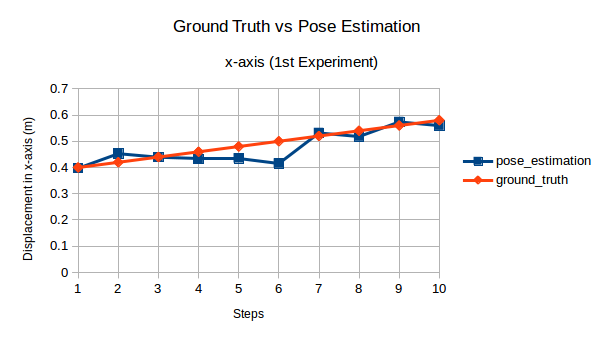
\includegraphics[width=5in, height=3.5in]{figures05/1_x_validation.png}
\caption{Ground Truth and Pose Estimation: x-axis ($1^{st}$ Experiment, Astra Camera)}
\label{fig:errorx_1nd}
\end{center}
\end{figure}
\begin{figure}[!h]
\begin{center}
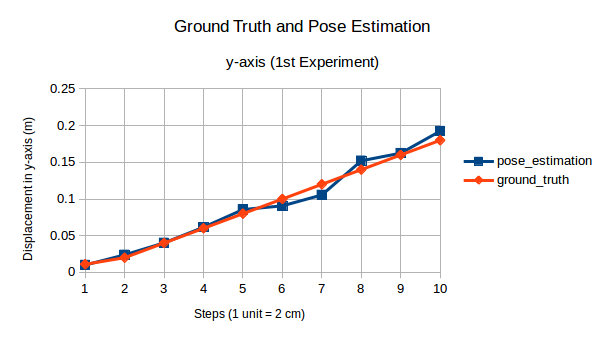
\includegraphics[width=5in, height=3.5in]{figures05/1_y_validation.png}
\caption{Ground Truth and Pose Estimation: y-axis ($1^{st}$ Experiment, Astra Camera)}
\label{fig:errory_1nd}
\end{center}
\end{figure}
\begin{figure}[!h]
\begin{center}
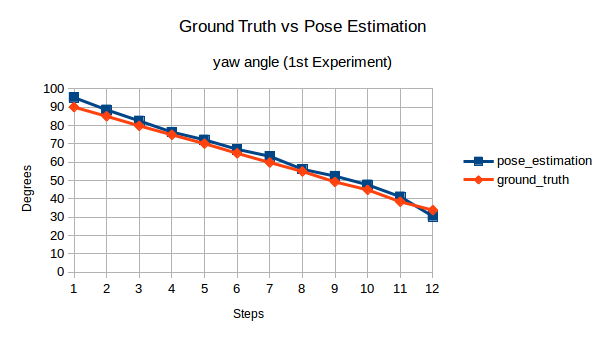
\includegraphics[width=5in, height=3.5in]{figures05/1_yaw_validation.png}
\caption{Ground Truth and Pose Estimation: yaw angle ($1^{st}$ Experiment, Astra Camera)}
\label{fig:erroryaw_1nd}
\end{center}
\end{figure}

For the case when the source cloud as well as the target cloud are generated from the sensory device as described in \ref{valitest}. Figures \ref{fig:errorx_2nd}, \ref{fig:errory_2nd}, and \ref{fig:erroryaw_2nd} were obtained for the second experiment. The graphs show that the estimated pose deviates slightly from its ground values.
%%%%%%%%%%%%%%%%%%%%%%%%%%%%% cloud from the same source
\begin{figure}[!h]
\begin{center}
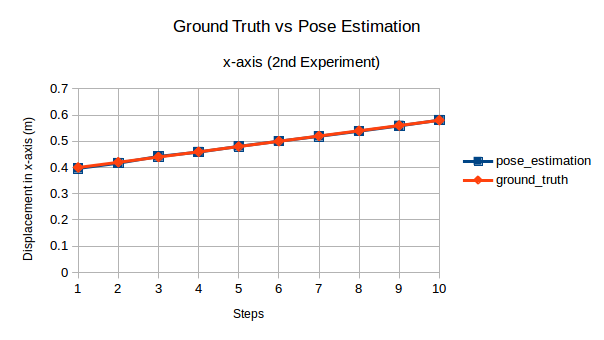
\includegraphics[width=5in, height=3.5in]{figures05/2_x_validation.png}
\caption{Ground Truth and Pose Estimation: x-axis ($2^{nd}$ Experiment, Astra Camera)}
\label{fig:errorx_2nd}
\end{center}
\end{figure}
\begin{figure}[!h]
\begin{center}
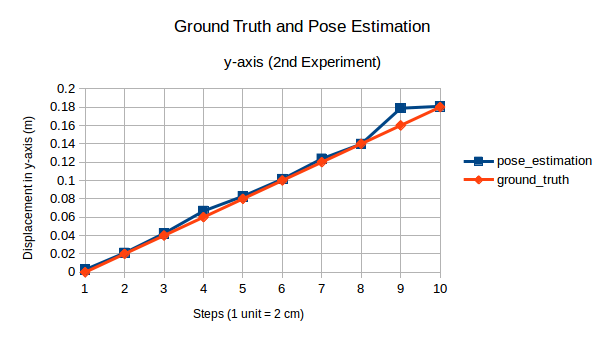
\includegraphics[width=5in, height=3.5in]{figures05/2_y_validation.png}
\caption{Ground Truth and Pose Estimation: y-axis ($2^{nd}$ Experiment, Astra Camera)}
\label{fig:errory_2nd}
\end{center}
\end{figure}
\begin{figure}[!h]
\begin{center}
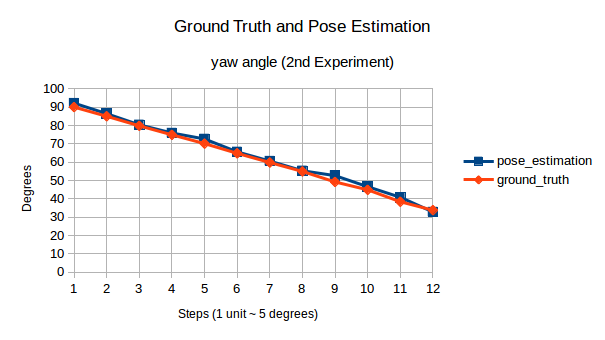
\includegraphics[width=5in, height=3.5in]{figures05/2_yaw_validation.png}
\caption{Ground Truth and Pose Estimation: yaw angle ($2^{nd}$ Experiment, Astra Camera)}
\label{fig:erroryaw_2nd}
\end{center}
\end{figure}

%%%%%%%%%%%%%%%%%%%%%%%%%%%
From the deviation graph an absolute error can be calculated. Figures \ref{fig:absx}, \ref{fig:absy} and \ref{fig:absw} show the error calculated for both experiments.

\begin{figure}[!h]
\begin{center}
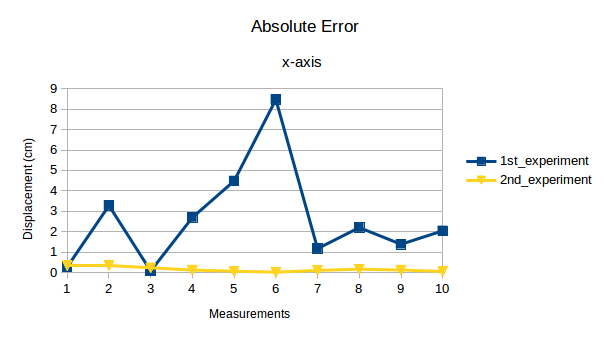
\includegraphics[width=5in, height=3.5in]{figures05/abs_error_x.png}
\caption{Absolute Error: x-axis}
\label{fig:absx}
\end{center}
\end{figure}

\begin{figure}[!h]
\begin{center}
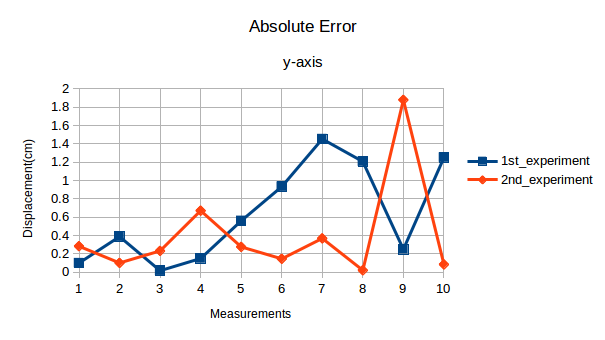
\includegraphics[width=5in, height=3.5in]{figures05/abs_error_y.png}
\caption{Absolute Error: y-axis}
\label{fig:absy}
\end{center}
\end{figure}

\begin{figure}[!h]
\begin{center}
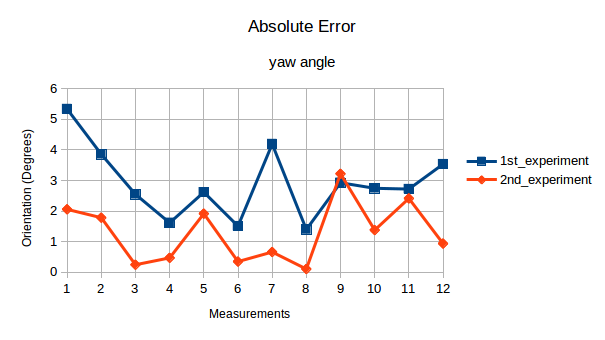
\includegraphics[width=5in, height=3.5in]{figures05/abs_error_yaw.png}
\caption{Absolute Error: yaw angle}
\label{fig:absw}
\end{center}
\end{figure}

\iffalse
meaning the solution did not register
\fi

\subsection{Result Analysis}

After analyzing the outcomes of the first experiment, it was concluded that the pose estimation did not perform well. Since the cloud generated from the CAD model did not converge to the cloud generated from the scene in several cases. This unsuccessful event can occur for several reasons. One of the reasons could be that in the matching process, the block that performs the coarse estimation of the object pose failed due to the lack of correspondence between the points clouds representing the CAD model and point clouds representing the scene. Another reason could be that, in the target cloud, noise and outlier were present, but in the source, they were not. In addition to that, the point cloud from the sensory device was too wavy (having a series of curves), as it was the case for the real sense camera where no results were reported. Figure Annex \ref{chap:pointclouds} shows the point clouds representing the industrial object, where the clouds were generated from the CAD model, RealSense camera and Astra camera.\\
Since the issue described previously was regularly present, it was concluded that matching a point cloud from the CAD model with a point cloud of a partial view of the scene was a difficult task to accomplish. A normal issue has already registered in most of the literature of the computer vision that deals with the task of estimation of object pose giving the CAD model and point cloud taken from domestic camera.	\\ 
With the issue encountered and briefly discussed above, the result was good enough provided that the camera used in the validation test was the Astra camera. Table \ref{absolute} shows an overall mean error of 2.6 cm for the x-axis, with a standard deviation; 2.45 cm, for the y-axis the overall mean error was 0,63 cm with a standard deviation; 0.5 cm and finally the orientation angle with an overall error of $2.9^{\circ}$ with a standard deviation of $1.27^{\circ}$. It can be concluded that the results are quite promising under the giving conditions, where a domestic camera was used during the whole thesis, and not an industrial one which would be suitable for this type of task. 

The second experiment is executed, where the source cloud needed to be changed. To accomplish that, a partial view of the scene is taken and used as a source cloud, which is fed to the pose estimation system in the offline stage as described in \ref{chap:theo}. The workaround may not be a proper solution since a partial view of the scene is taken into account, but it was proved to be good enough according to the output from the pose estimation system. An ideal solution would require the whole reconstruction of the 3D object with the camera to be used and then to render the object in order to prove the robustness of the system for different views. But it proved to be quite laborious since special hardware as well as software, needed to be implemented. For the purpose of the thesis, where an isolated object needed to be taken, free of occlusion and clutter scene, this approach has been proven successful.

In Table \ref{absolute}, the absolute error values calculated for the second experiment are shown. It clearly shows an improvement when the source cloud generated from the CAD was replaced for a point cloud representing a partial view of the scene. It reports an overall mean value for the x-axis of 0.152 cm,  with standard deviation of 0.1134 cm. For the y-axis reported an overall mean error of 0.406[cm] with a standard deviation of 0.5492 cm. As to the orientation around the z-axis, an overall mean of $1.21^{\circ}$ with a standard deviation of $1.019^{\circ}$ was reported. It was proved satisfactory that the pose estimation system performed successfully as long as the source cloud and target cloud are generated from the same sensory device, which in our case, was the Astra camera. It is also concluded, from the validation tests, that the RealSense camera is not suitable for this type of task where a reasonable quality of point cloud is needed.  


\begin{table}[ht]
\renewcommand{\arraystretch}{1.3}
\caption{Absolute Error Values (Astra Camera).}
\label{absolute}
\centering
\begin{tabular}{|c||c||c||c||c|}
\hline
  & Mean (1st Exp)& STD &  Mean (2nd Exp )& STD \\
\hline
x-axis (cm) & 2.6052 & 2.4562 & 0.1520 & 0.1134\\
\hline
y-axis (cm) & 0.6306 & 0.5354 & 0.4062 & 0.5492\\
\hline
yaw angle (degrees)& 2.8748 & 1.2741 & 1.2177 & 1.0197\\
\hline
\hline
\end{tabular}
\end{table}


